\documentclass[12pt,a4paper]{article}
%\usepackage{xcolor} \pagecolor[rgb]{0.5,0.5,0.5} \color[rgb]{1,1,1}
%\usepackage[utf8]{inputenc}
\usepackage[shortlabels]{enumitem}
%\usepackage{bm}
\usepackage{mathrsfs}
\usepackage{amsmath}
\usepackage{amssymb}
\usepackage{hyperref}
\usepackage{graphicx}
\begin{document}
\title{Solutions to BDA Assignment 1,
 2020/2021 Semester 2}
\author{Theodoros Ladas, s2124289}
\date{\today}
\maketitle

\vspace{1cm}

\noindent\textbf{1)}
\begin{enumerate}[(a)]
%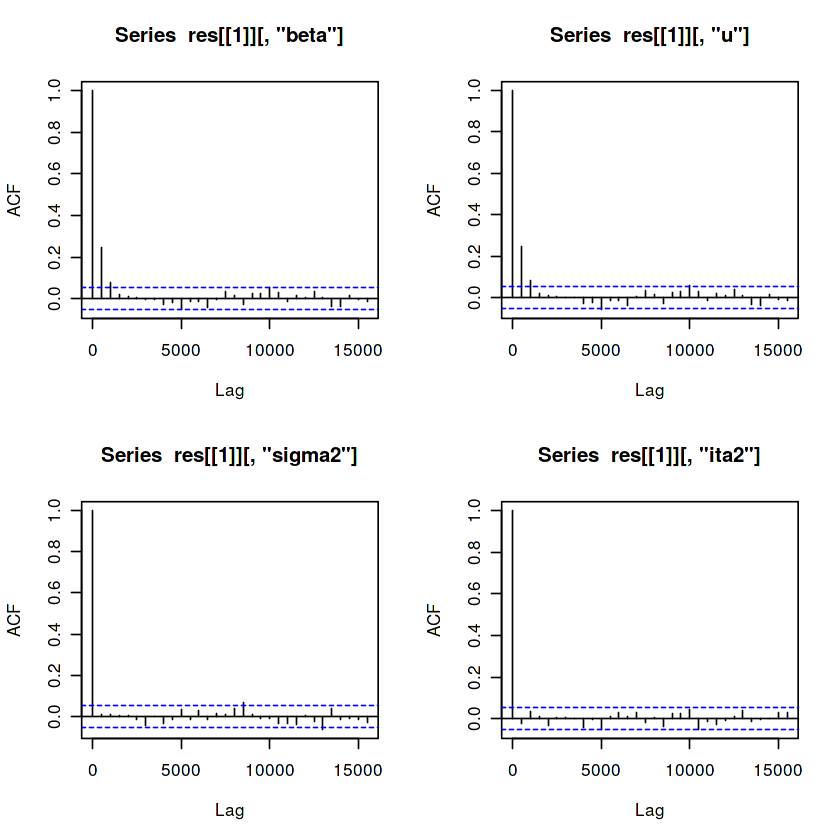
\includegraphics[scale=0.3]{./images/1_Figure0.png}
\item

Explanation: A state-space model is built in this assignment in order to model the population (log-population) of whales, with data from 1952 up to 1997. The model is divided into the state model 
$x_t = b x_{t-1}+u+w_t; \quad w_t\sim N(0,\sigma^2)$, and an observation model $y_t =x_{t}+v_t, \quad v_t\sim N(0,\eta^2)$. Here the meaning of the parameters of the model will be discussed, specifically, $b, u, \sigma^2, \eta^2$. 

The $b$ parameter, is the coefficient that connects the previous log-population, to the current one. In other words, if there is no noise on our data, therefore the relationship being completely deterministic, the log-population of the whales would change from $t=i$ to $t=i+1$ by $b$. 

The $u$ parameter, is the intersect of the state model, and its interpretation is: $u$ would be the log-population of whales at time $t=0$.

The $\sigma^2$ parameter, is the parameter of the variance of random noise of the underlying state model discribed above. 

Finally, the $\eta^2$ parameter, has a similar explanation to the $\sigma^2$ parameter as it also is the parameter of variance of random noise, but this time it represents the noise of the observation equation. That means that even if our underlying model was deterministic, there is also an extra uncertainty in our model, because of the observation error that might occur.

The point of modeling the log-population of whales with this state-space model, is that now, we can have priors on all this parameters, that are going to be updated from our dataset in later stages. 

\item
Explanation: The dataset had some missing values that needed to be addressed before continuing with building the engine of the model. First of all the missing data came in two different ways, first of all, there where years in the dataset where the popuplation observed was reported as NA, and secondly there where missing years from the data, indicating that the observed population for that year, is NA. On the first group, no additional imputation step was taken, because the model was going to be evaluated using JAGS (Just Another Gibbs Sampler). JAGS, treats these kinds of NAs as stochastic nodes, meaning that they are another part of our model. On the other had, the second kind of NAs, was treated by injecting into the dataset the years that where completely missing allong with an NA for the observed population value.

The priors for the model are stated here. It was assumed that $x_0 \sim N(\text{log}(2500),1)$, $b \sim U(0,1)$, $u \sim \text{exp}(1)$ and finaly, $\sigma^2, \eta^2 ~ \text{inv-Gamma}(0.1,0.1)$

The burn in period for which the data are discarded for computing estimated of these parameters, was selected to be $2,000$ iterations, and the whole simulation run for $700,000$ iterations.

\item
Explanation: In order to check the mixing of the chains, the Gelman-Rubin statistic was calculated. The Diagrams below, show this statistic per iteration. One idicates that there is no evidence that show a problem of the mixing of the chains. We can see that on iteration $700,000$ the statistic is either at one, of very close to it ($1.01$) for all the parameters of the model, so this is a good sign. Also, a second way that the mixing of the chains was evaluated, was by the autocorrealtion plots. These are shown below as well per parameter. What we can observe is that for the first iteration the autocorrelation is $1$, which is expected since we are using a Markov-Chain model. However, either on the second lag, or very quicly after that the autocorrelation of the point explored by the algorithm, versus the previous one, goes to $0$ and stays there. That is also a very good indication that the algorithm is not 'stuck' on a small space of the parameter space and instead explores the whole space. 

Results:

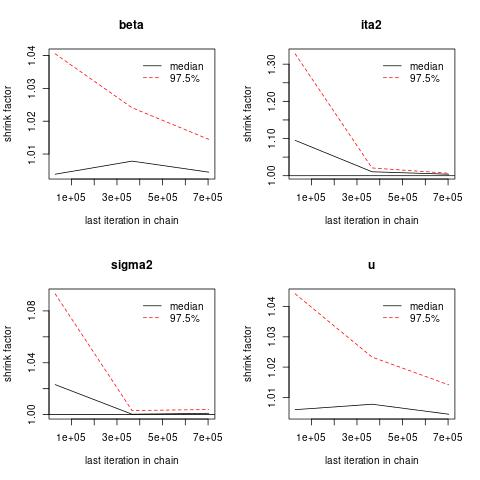
\includegraphics[scale=0.44]{./images/1_Figure00_gelman.jpg}
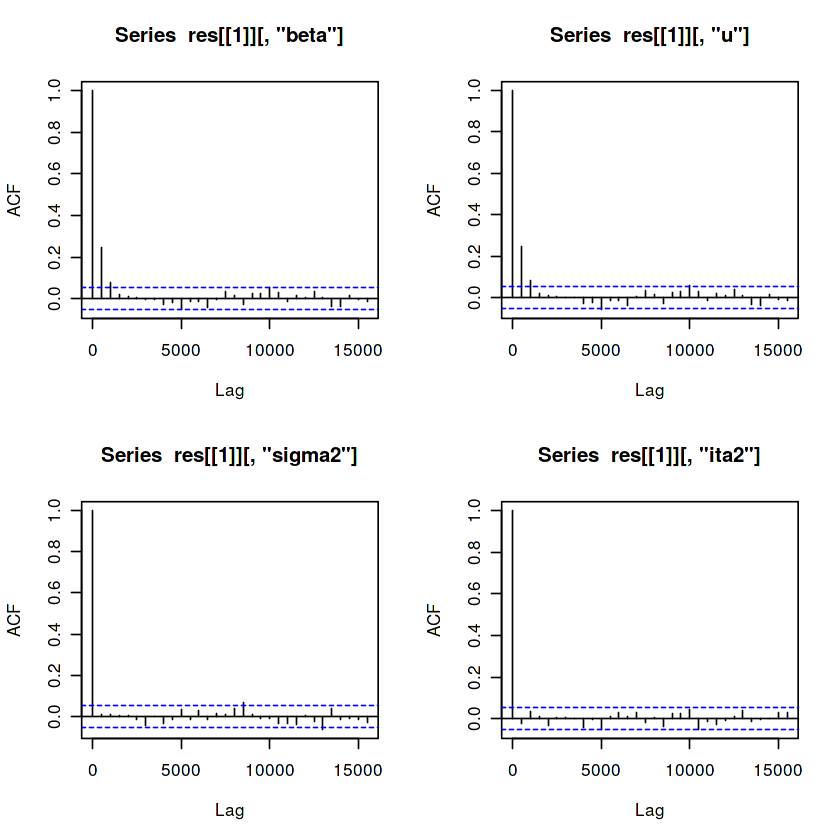
\includegraphics[scale=0.25]{./images/1_Figure0.png}

\item
Explanation: Here the results from the above simulation are presented. 

\includegraphics[scale=0.25]{./images/1_Table0.png}

We can see that the mean and standard deviation values for all the parameters, as well as confidence intervals for each parameter.

Below the plot of the posterior densities and their prior densities are also plotted. From these diagrams we can clearly see that the prior is not dominating the posterior in any case, so our choice of prior densities and hyperparameters is reasonable. In order to further robustify the method, later a sensitivity analysis, will be performed.

Results:

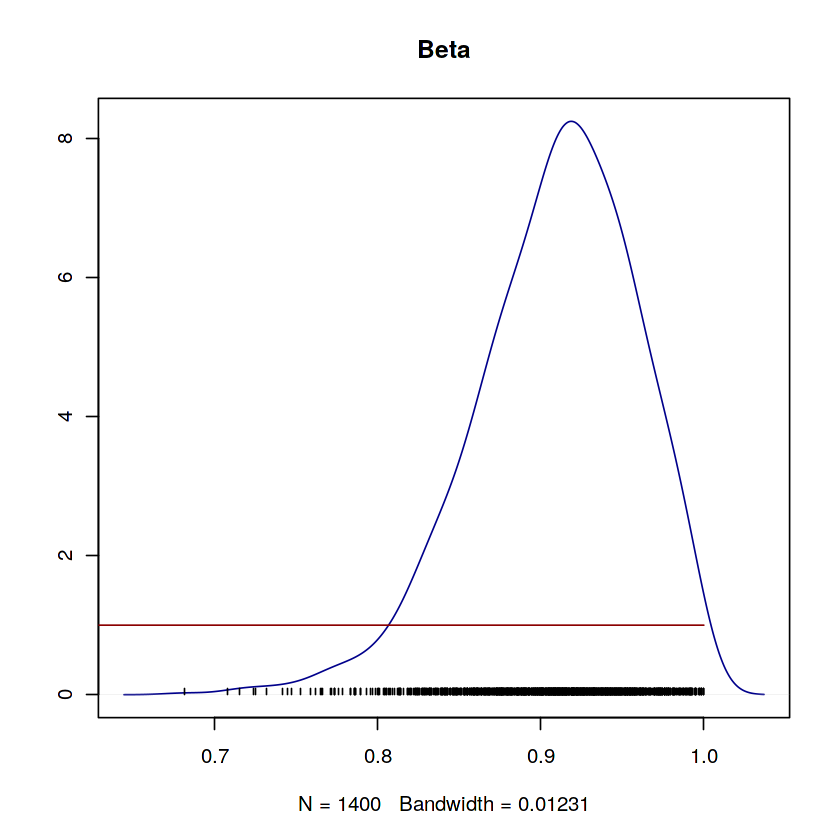
\includegraphics[scale=0.25]{./images/1_Figure3_beta_posterior.png}
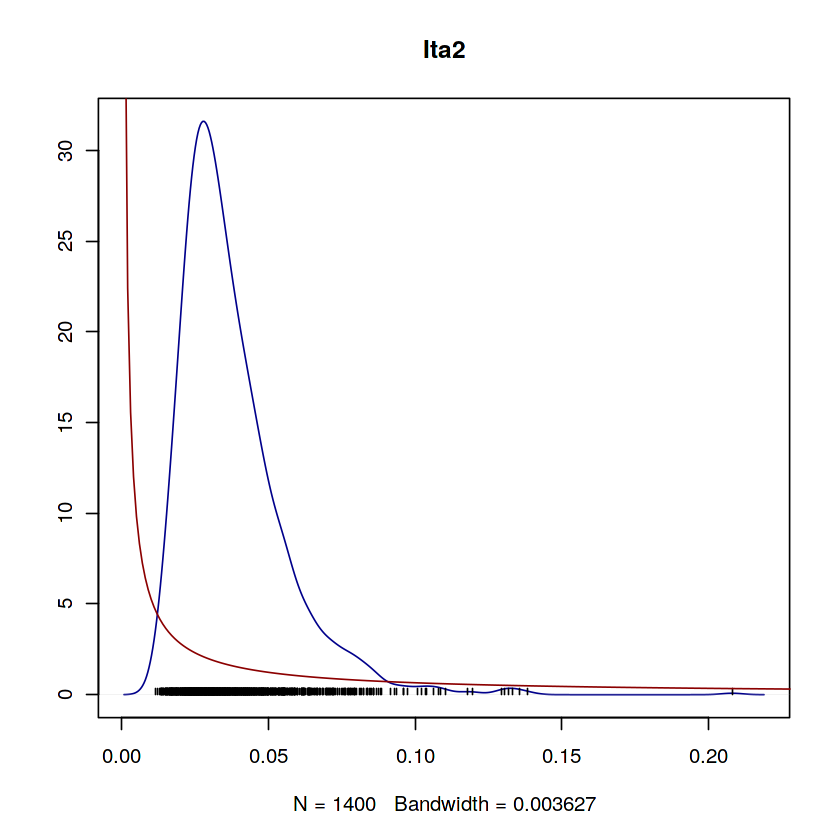
\includegraphics[scale=0.25]{./images/1_Figure3_ita_posterior.png}


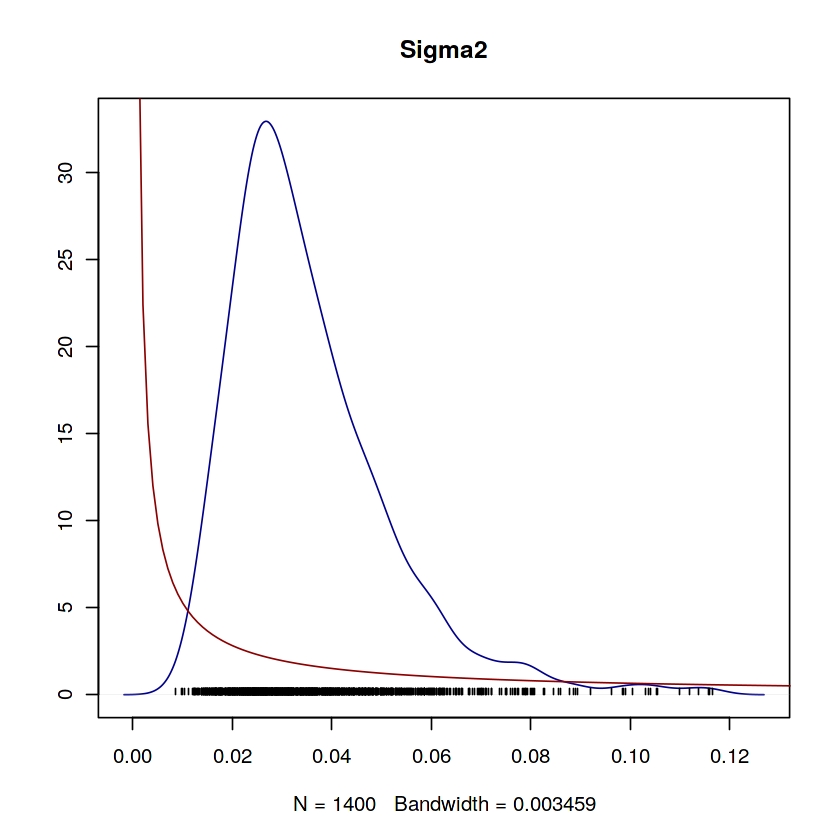
\includegraphics[scale=0.25]{./images/1_Figure3_sigma_posterior.png}
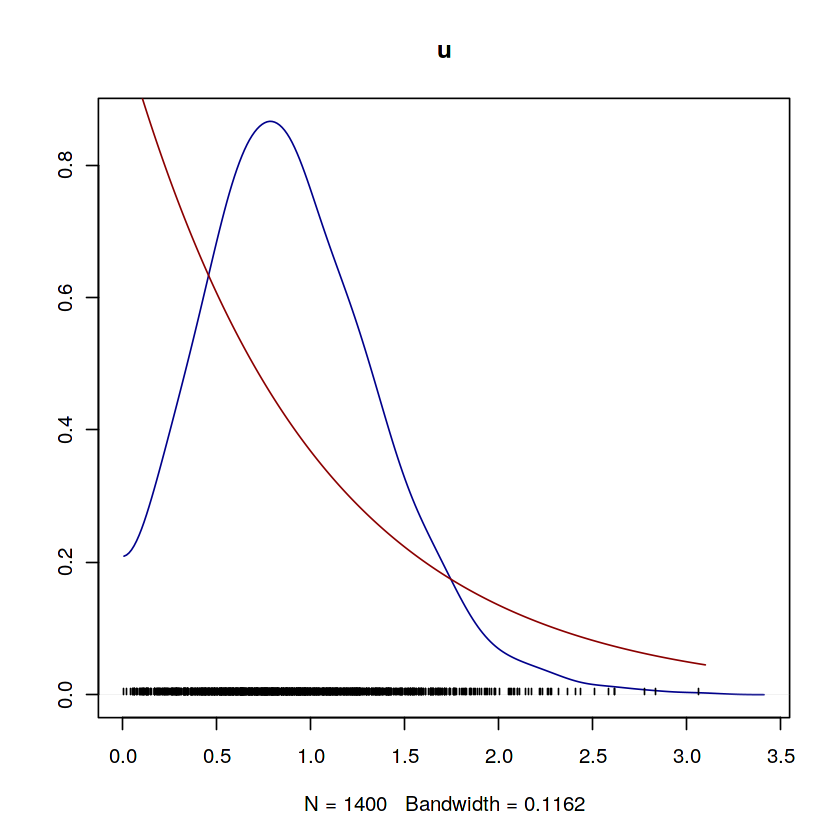
\includegraphics[scale=0.25]{./images/1_Figure3_u_posterior.png}

\item
Explanation: Here the sensitivity analysis is discussed. The priors where chosen as follows. The distribution for the prior of each parameter stayed the same and the choice of starting hyperpareters was vastly different, in order to see whether the results will change or not.
More specifically, $b \sim U(-1,2)$, $u \sim \text{exp}(3)$ and finaly, $\sigma^2, \eta^2 ~ \text{inv-Gamma}(1/0.1,1/0.1)$. The prior for $x_0$ stayed the same. 

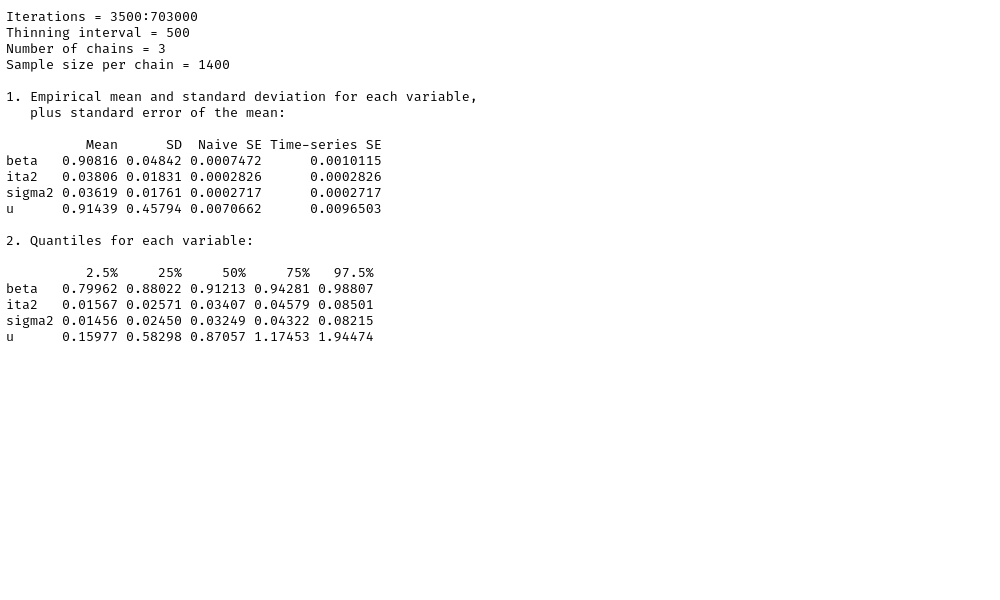
\includegraphics[scale=0.25]{./images/1_table1.png}

As we can see the results changed to the fourth significant digit. This clearly idicated that the prior doesn't dominate the posterior and it makes it even more likely that the posterior density is converging to the true value of the parameters. The autocorellation plot figure for this model is also present in the results graph, used as in the first model to check the mixing of the new chains.

Results:

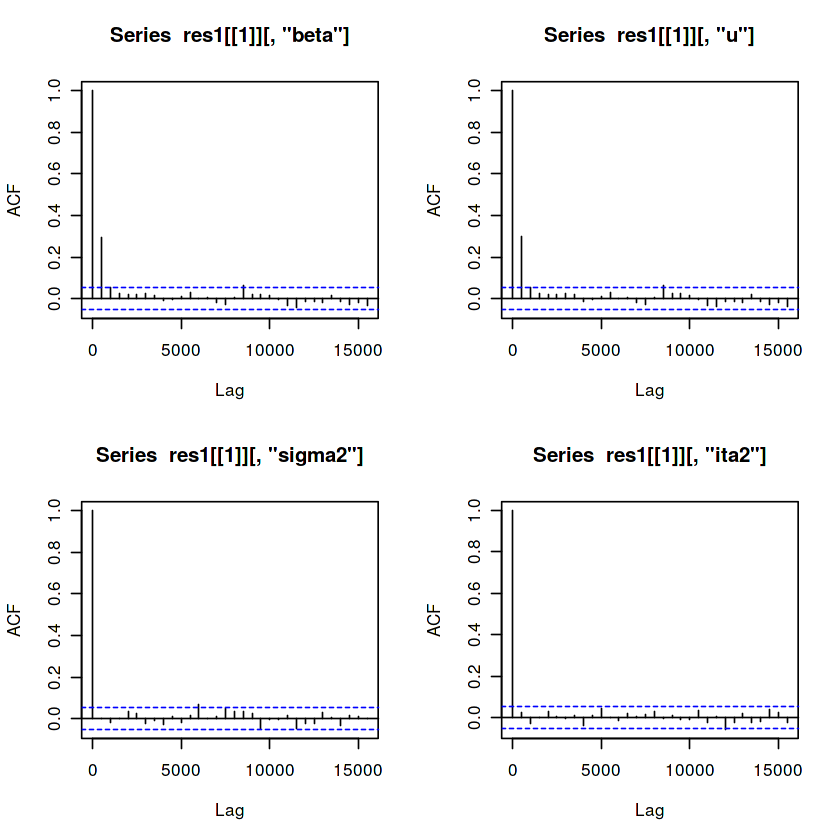
\includegraphics[scale=0.30]{./images/1_Figure4_acf.png}

\item
Explanation: On the below graph, the evolution of the posterior mean of log-population of whales is presented. This line is projected to 2050. The dotted lines show the 95\% Confidence intervals (the lower line is the 2.5\% and the upper line the 97.5\%). We see that the mean get's stable after a while, which is what we expected since the $\beta$ coefficient was around $0.9$. A $\beta$ of $1$ idicates a stationary process in the AR(1) model. We also see the 95\% CI for the mean to diverge very heavily. This is because our last observed datapoint is in 1997 and we are trying to predict 2050. This divergence explained because the state-model has a random noise and the observed values model has another small random noise. All these 'mistakes' add up, making the projection for 2050 have a very big variance associated with it.
Also the posterior probability that the population of gray whales becores smaller than 100 at any year from 1951 until the end of 2050 was calculated to be 0. Or mathematically, $p(\min_{t\in \{0,1\ldots,99\}} x_t<=\log(100)|y) = 0$

Results:

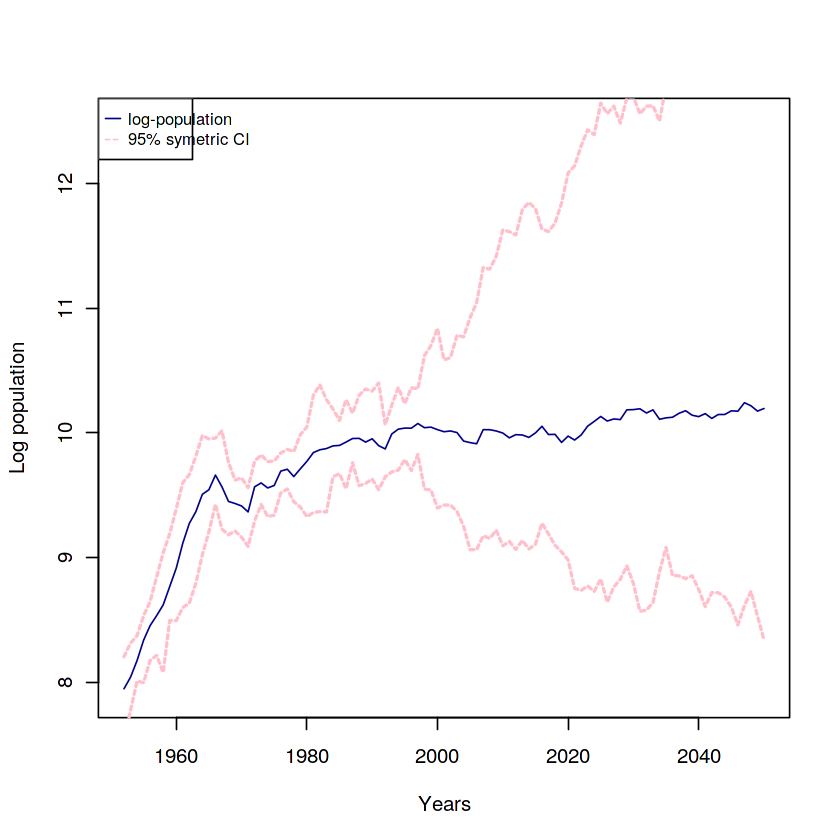
\includegraphics[scale=0.25]{./images/1_Figure5_final_plot.png}


\item
Explanation: Finally, posterior predictive checks for various statistics, specifically, the min, the max and the mean, to evaluate the fit of this model, where the prior are the original ones stated in section (b) was performed. The results are reported below in the form of histograms of the posterior predictive samples generated from the model. The red lines indicate the min, the max and the mean of the given sample that we observed respectively. We can clearly see that in all cases the line is well within the bounds of the histograms. The most extreme case is that of the min, but even this is still acceptable as it is within $2 \sigma$ from the mean of its distribution.

Results:

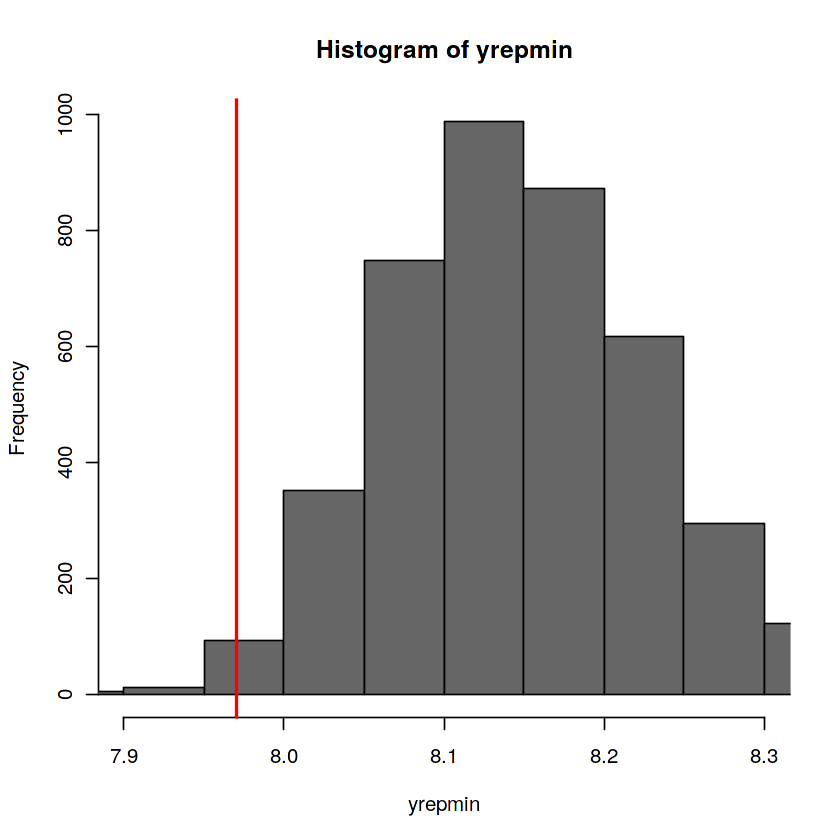
\includegraphics[scale=0.17]{./images/1_Figure6_predictive_0.png}
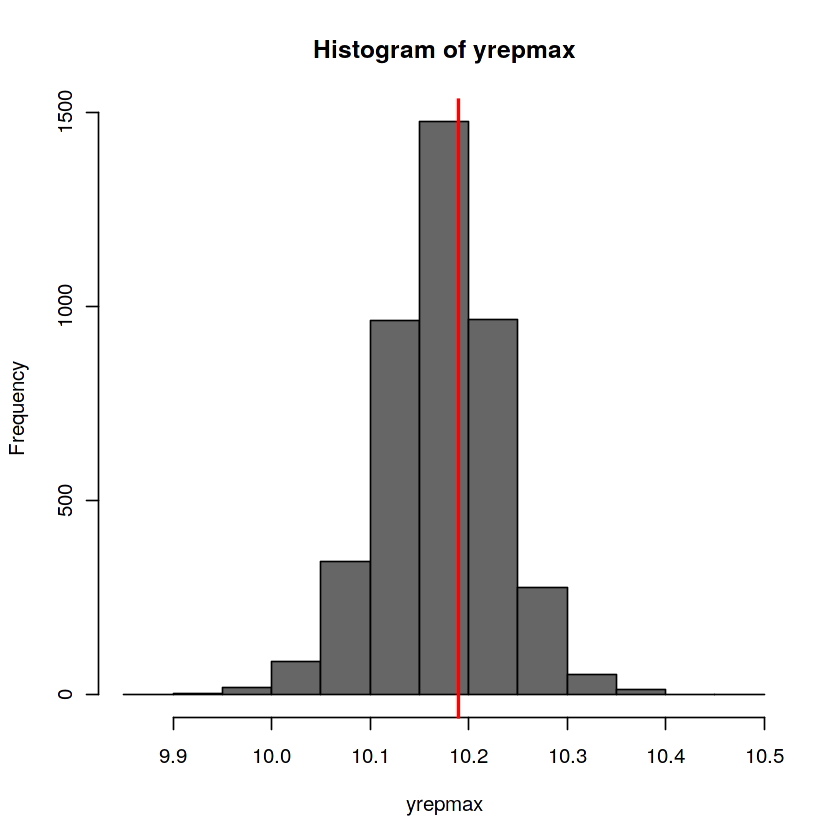
\includegraphics[scale=0.17]{./images/1_Figure6_predictive_1.png}
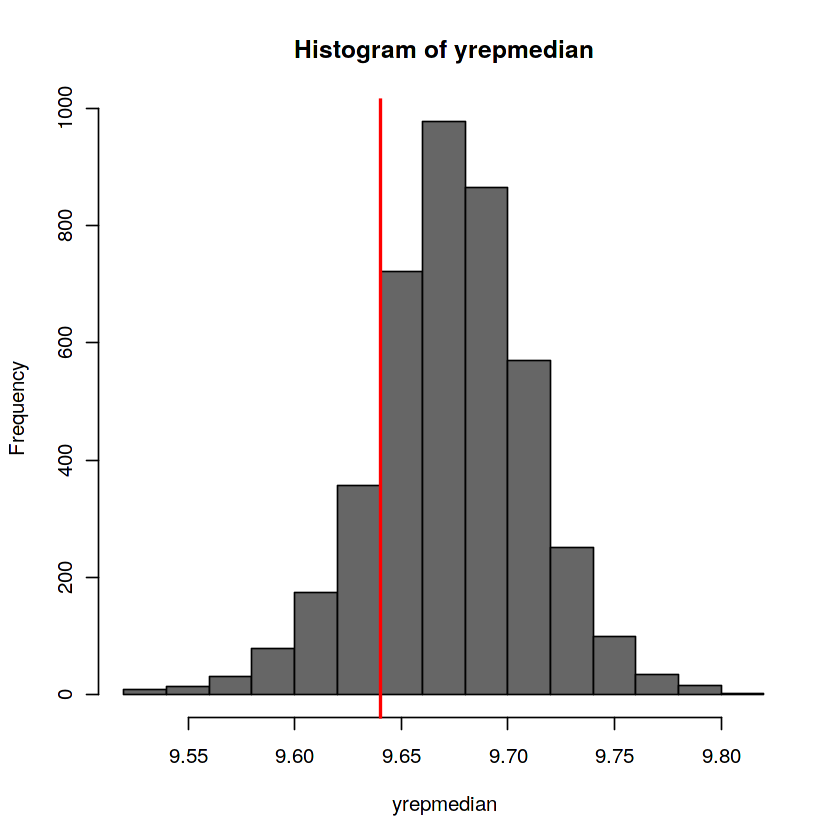
\includegraphics[scale=0.17]{./images/1_Figure6_predictive_2.png}



\end{enumerate}

\noindent\textbf{2)}
\begin{enumerate}[(a)]
\item
Explanation:

Results:

\item
Explanation:

Results:

\item
Explanation:

Results:

\item
Explanation:

Results:

\item
Explanation:

Results:

\item
Explanation:

Results:

\item
Explanation:

Results:

\end{enumerate}
\end{document}